\documentclass[border=10pt]{standalone}
\usepackage{tikz}
\usetikzlibrary{arrows.meta, patterns, calc, positioning}

\begin{document}
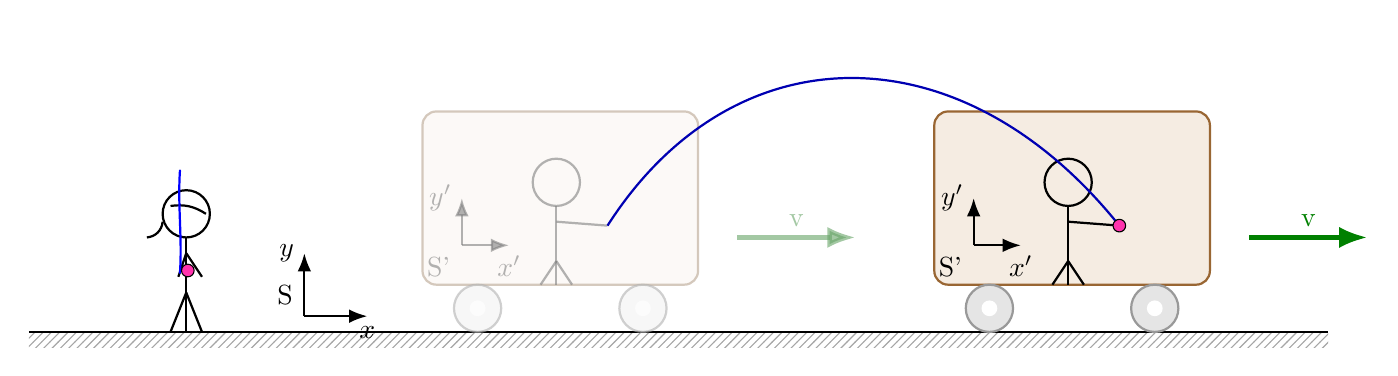
\begin{tikzpicture}[
    >=Latex,
    axis/.style={->, thick},
    person/.style={thick, black},
    faded person/.style={thick, gray},
    cart border/.style={draw=brown!80!black, thick, rounded corners=5pt},
    cart fill/.style={fill=brown!15},
    faded cart border/.style={draw=brown!60!black!50, thick, rounded corners=5pt},
    faded cart fill/.style={fill=brown!15!white!50},
    wheel/.style={draw=gray!80, fill=gray!20, thick, circle},
    faded wheel/.style={draw=gray!60, fill=gray!10, thick, circle},
    velocity/.style={->, ultra thick, green!50!black},
    faded velocity/.style={->, ultra thick, green!40!black!60},
]

% Ground
\pattern[pattern=north east lines, pattern color=gray!70] (-3, -0.2) rectangle (13.5, 0);
\draw[thick] (-3, 0) -- (13.5, 0);

% --- Stationary Frame S ---
\coordinate (S_origin) at (0.5, 0.2);
\node[above left=1pt of S_origin] {S};
\draw[axis] (S_origin) --++ (0.8, 0) node[below] {$x$};
\draw[axis] (S_origin) --++ (0, 0.8) node[left] {$y$};

% Stationary Observer (Alice)
\begin{scope}[shift={(-1, 0.5)}, person]
    % Body and legs
    \draw (0, -0.5) -- (0, 0.7); % Torso
    \draw (0, 0) -- (0.2, -0.5); % Right leg
    \draw (0, 0) -- (-0.2, -0.5); % Left leg
    % Head and hair
    \draw (0, 1) circle (0.3);
    \draw (-0.2, 1.1) to[bend left=20] (0.25, 1.0); % Fringe
    \draw (-0.3, 0.9) to[bend left=40] (-0.5, 0.7); % Ponytail
    % Arms and projectile path
    \draw (0, 0.5) -- (0.2, 0.2); % Left arm (free)
    \coordinate (saber_pos) at (-0.1, 0.2);
    \draw (0, 0.5) -- (saber_pos); % Right arm
    \draw[blue, line width=0.8pt, line cap=round] ($(saber_pos)+(0.02,0.05)$) .. controls +(0.03,0.45) and +(-0.03,-0.45) .. ($(saber_pos)+(0.02,1.35)$);
    \fill[red!40!magenta!80, draw=black, thin] ($(saber_pos)+(0.12,0.08)$) circle (0.08);
\end{scope}

% --- Moving Frame S' ---

% Define cart dimensions
\def\cartw{3.5}
\def\carth{2.2}
\def\wheelr{0.3}
\def\bodyraise{0.6}

% Initial Position (faded)
\begin{scope}[opacity=0.6]
    \coordinate (cart1_pos) at (2, 0);
    
    % Cart body
    \draw[faded cart border, faded cart fill] ($(cart1_pos)+(0,\bodyraise)$) rectangle ++(\cartw, \carth);
    
    % Wheels
    \coordinate (wheel1a) at ($(cart1_pos) + (0.7, \wheelr)$);
    \coordinate (wheel1b) at ($(cart1_pos) + (\cartw-0.7, \wheelr)$);
    \draw[faded wheel] (wheel1a) circle (\wheelr);
    \fill[white] (wheel1a) circle (0.1);
    \draw[faded wheel] (wheel1b) circle (\wheelr);
    \fill[white] (wheel1b) circle (0.1);
    
    % Observer inside (Bob 1)
    \coordinate (bob1_pos) at ($(cart1_pos) + (1.7, \bodyraise)$);
    \begin{scope}[shift={(bob1_pos)}, faded person]
        \draw (0, 0) -- (0, 1); % Torso
        \draw (0, 0.3) -- (0.2, 0); % Right leg
        \draw (0, 0.3) -- (-0.2, 0); % Left leg
        \draw (0, 1.3) circle (0.3); % Head
        \coordinate (hand1) at (0.65, 0.75);
        \draw (0, 0.8) -- (hand1); % Arm
    \end{scope}
    
    % S' frame
    \coordinate (Sprime1_origin) at ($(cart1_pos) + (0.5, \bodyraise+0.5)$);
    \node[below left=1pt of Sprime1_origin, gray] {S'};
    \draw[axis, gray] (Sprime1_origin) --++ (0.6, 0) node[below, gray] {$x'$};
    \draw[axis, gray] (Sprime1_origin) --++ (0, 0.6) node[left, gray] {$y'$};
    
    % Velocity vector
    \draw[faded velocity] ($(cart1_pos) + (\cartw+0.5, \bodyraise+0.6)$) --++ (1.5, 0) node[midway, above] {v};
\end{scope}

% Final Position (solid)
\begin{scope}
    \coordinate (cart2_pos) at (8.5, 0);
    
    % Cart body
    \draw[cart border, cart fill] ($(cart2_pos)+(0,\bodyraise)$) rectangle ++(\cartw, \carth);
    
    % Wheels
    \coordinate (wheel2a) at ($(cart2_pos) + (0.7, \wheelr)$);
    \coordinate (wheel2b) at ($(cart2_pos) + (\cartw-0.7, \wheelr)$);
    \draw[wheel] (wheel2a) circle (\wheelr);
    \fill[white] (wheel2a) circle (0.1);
    \draw[wheel] (wheel2b) circle (\wheelr);
    \fill[white] (wheel2b) circle (0.1);
    
    % Observer inside (Bob 2)
    \coordinate (bob2_pos) at ($(cart2_pos) + (1.7, \bodyraise)$);
    \begin{scope}[shift={(bob2_pos)}, person]
        \draw (0, 0) -- (0, 1); % Torso
        \draw (0, 0.3) -- (0.2, 0); % Right leg
        \draw (0, 0.3) -- (-0.2, 0); % Left leg
        \draw (0, 1.3) circle (0.3); % Head
        \coordinate (hand2) at (0.65, 0.75);
        \draw (0, 0.8) -- (hand2); % Arm
    \end{scope}
    
    % S' frame
    \coordinate (Sprime2_origin) at ($(cart2_pos) + (0.5, \bodyraise+0.5)$);
    \node[below left=1pt of Sprime2_origin] {S'};
    \draw[axis] (Sprime2_origin) --++ (0.6, 0) node[below] {$x'$};
    \draw[axis] (Sprime2_origin) --++ (0, 0.6) node[left] {$y'$};
    
    % Velocity vector
    \draw[velocity] ($(cart2_pos) + (\cartw+0.5, \bodyraise+0.6)$) --++ (1.5, 0) node[midway, above] {v};
\end{scope}

% Trajectory and Ball
\draw[blue!70!black, thick] (hand1) .. controls +(1.6,2.5) and +(-2.0,2.5) .. (hand2);
\fill[red!40!magenta!80, draw=black, thin] (hand2) circle (0.08);

\end{tikzpicture}
\end{document}
